\documentclass{report}

\usepackage{physics}
\usepackage{graphicx}
\usepackage{hyperref}

\usepackage{listings}
\usepackage{color}

\definecolor{red}{rgb}{1,0,0}
\definecolor{dkgreen}{rgb}{0,0.6,0}
\definecolor{gray}{rgb}{0.5,0.5,0.5}
\definecolor{mauve}{rgb}{0.58,0,0.82}

\renewcommand{\thesection}{\arabic{section}}
\setcounter{secnumdepth}{3}
\setcounter{tocdepth}{3}

\hypersetup{
    colorlinks=true,
    linkcolor=blue,
    filecolor=magenta,      
    urlcolor=blue,
}

\lstset{
    frame=tb,
    language=Python,
    aboveskip=3mm,
    belowskip=3mm,
    showstringspaces=false,
    columns=flexible,
    basicstyle={\small\ttfamily},
    numbers=none,
    numberstyle=\tiny\color{gray},
    keywordstyle=\color{blue},
    commentstyle=\color{dkgreen},
    stringstyle=\color{mauve},
    breaklines=true,
    breakatwhitespace=true,
    tabsize=3
}

\title{COVID-19 Data Analysis}

\author{Rishav Bhagat}

\graphicspath{{../res/imgs/}}

\begin{document}
    \maketitle
    \tableofcontents
    \newpage
    \section{Dataset}
        I used the dataset that was collected and used by John Hopkins University for 
        \href{https://www.arcgis.com/apps/opsdashboard/index.html#/bda7594740fd40299423467b48e9ecf6}{this project}. 
        This dataset was collected from many international health organizations and all compiled into onto github repository. 
        It contains information on daily reports (including new cases, deaths, and recoveries), and global trends. 
        \newline \indent
        Here is the link to the datasets I used: 
        \newline\indent\indent \href{https://github.com/CSSEGISandData/COVID-19}{https://github.com/CSSEGISandData/COVID-19}
        \subsection{Downloading the Data}
            I created a batch script to download all this data using git, delete files that are not needed for my analysis, and move the files into more convienient locations.
            \begin{lstlisting}
                @echo off
                rmdir data /s /q
                git clone https://github.com/CSSEGISandData/COVID-19.git
                rename COVID-19 data
                cd data
                rmdir .git /s /q
                rmdir archived_data /s /q
                rmdir who_covid_19_situation_reports /s /q
                del README.md
                mv csse_covid_19_data/* .
                rmdir csse_covid_19_data /s /q
                cd ..
                git add data
                git commit -m "updated data from John Hopkins github repo"
                git push
            \end{lstlisting}
        \subsection{Initial Glance}
            First, I plotted the global coronavirus data (cases vs days) in a similar fashion to the way it was plotting on the John Hopkins project. This is to reveal any obvious trends.
            \begin{center}
                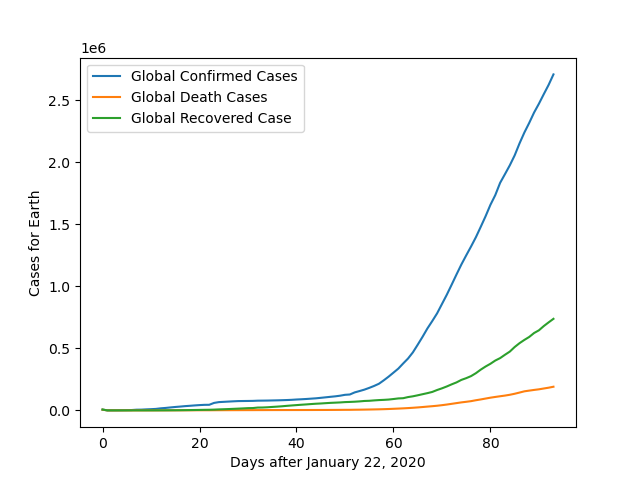
\includegraphics[width=10cm]{plots/global/cases.png}
            \end{center}
            At a first glance, this looks like exponential growth, so I then plotting a logarithmic graph with a line of best-fit.
            \begin{center}
                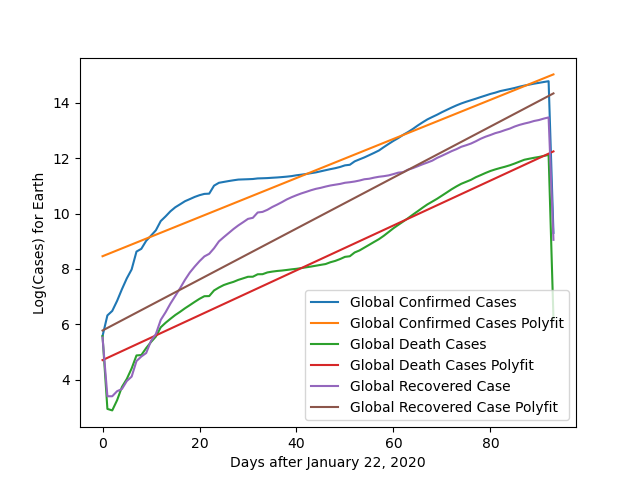
\includegraphics[width=10cm]{plots/global/log(cases).png}
            \end{center}
            A linear relationship in the logarithmic graph corresponds to an exponential relationship in the original graph. As we can see, the logarithmic graph is approximately linear, which confirms that so far, the coronavirus is exponentially growing. But we also see that the curve is beginning to flatten out, corresponding to the true logistic growth of the original graph. The beginning of all logarithmic graphs appear to be exponential, which explains why it apears as it does. 
            \newline
            \indent Now, we know that logistic growth will eventually level out, and it is in our interest to see when and where it will do this globally. We can do this by tracking the growth rate of the graph, as we shall see in the next section. 
    \section{Data Analysis and Implications}
        \indent First let's define some variables:
        \begin{itemize}
            \item Let us refer to the region we are talking about as $X$. For now $X$ refers to the entire globe.
            \item Let $N^X$ be the current number of people who have COVID-19 within $X$. I may sometimes just use $N$, which will refer to the region in question at the time.
            \item Let $N^X_i$ be the current number of people who have COVID-19 within $X$ on the $i$-th day after January 22nd (which is when John Hopkins began collecting data).
            \item Let $\Delta N^X_i = N^X_i - N^X_{i - 1}$ be the number of new cases on a given day, defined by $i$.
        \end{itemize}
        \subsection{Growth Rate}
            Now we can define our growth rate as 
            \begin{equation}
                G^X_i = \dfrac{\Delta N^X_i}{\Delta N^X_{i - 1}}
            \end{equation}
            We are interested when this value crosses from $G > 1$ to $G < 1$, which corresponds to a point of infection. It is when the numbers of new cases each day begins to decrease rather than increase. Or in terms of calculus, when the second derivative becomes negative. The reason we do not just use the second derivative is that this data is noisy and approximating a high-order derivative would not work too well. Now plotting the growth rate:
            \begin{center}
                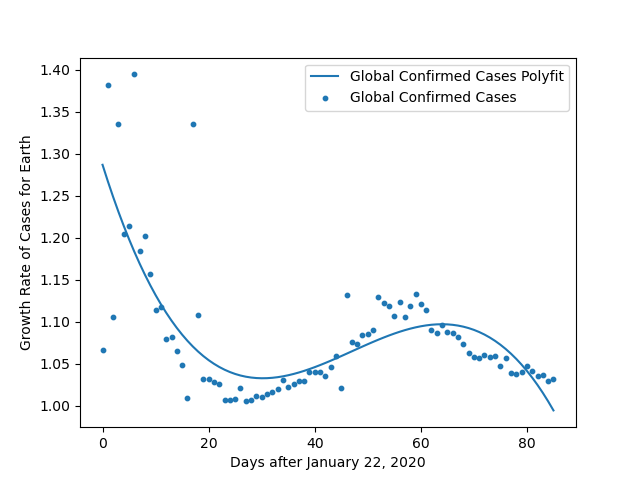
\includegraphics[width=10cm]{plots/global/growth_rate.png}
            \end{center}
            If the graph continues to follow the polyfit curve drawn, then we expect the inflection point to occur soon, but we do not know if it will go back up as it did at around $i = 25$. In fact, we can expect it to go up, which is evident by plotting the approximated derivative
            \footnote{
                When I refer to the derivative I am using the central difference approximation give by:
                $$f'(x) \approx \dfrac{f(x + h) - f(x - h)}{2h}$$
                with $h = 1$ since we have a discrete input space (each day).
            } of the growth function.
            \begin{center}
                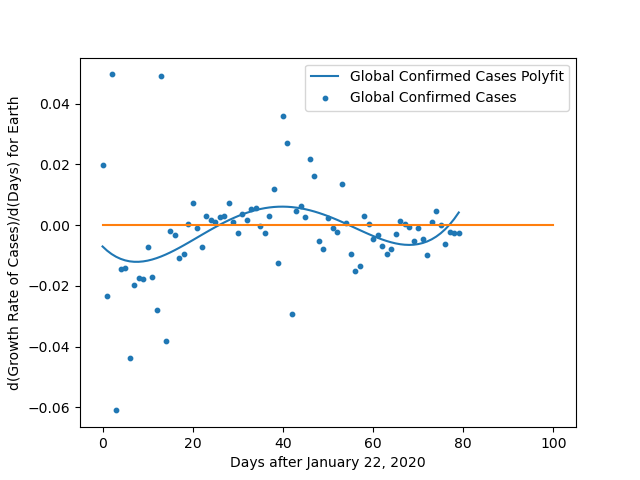
\includegraphics[width=10cm]{plots/global/growth_rate_derivative.png}
            \end{center} 
            The derivative of the growth rate at the current time ($i \approx 80$) is following the same pattern as at $i = 25$ and it has gone above the zero-line, implying that the growth rate will increase again.
            \newline
            \indent This is a dissapointing result since finding the true point of inflection will let us estimate where the number of cases will max out. If the point of inflection occurs at $i$, then it is reasonable to guess that the number of cases will max at $2 * N^X_i$ by the way logistic growth works.
            \subsubsection{Modelling with the Growth Rate}
                The curve generated by \lstinline{np.polyfit} fits the growth rate pretty well, so it may be possible to create a model based on the growth rate. To do so, we just have to follow the definitions of the growth rate and the solve for $N_i$:
                \begin{align*}
                    G^X_i = \dfrac{\Delta N^X_i}{\Delta N^X_{i - 1}} = \dfrac{N^X_i - N^X_{i - 1}}{N^X_{i - 1} - N^X_{i - 2}} \\
                    G^X_i(N^X_{i - 1} - N^X_{i - 2}) = N^X_i - N^X_{i - 1}
                \end{align*}
                and finally
                \begin{equation}
                    N^X_i = N^X_{i - 1} + G^X_i(N^X_{i - 1} - N^X_{i - 2})
                \end{equation}
                But there are a lot of problems with a model like this. For one it is based on previous estimates, so any error in early estimates will propagate through to the later estimates, making the model extremely inaccurate for anything too far out of the domain of the data.
                \newline
                \indent Also, as we showed before, the growth rate will likely not follow the polyfit curve outside the domain of the data.
        \subsection{Growth Ratio}
            Another intrinsic value to 
        \subsection{Derivative}
        \subsection{Fitting Polynomials to Subsets of the Data}
        \subsection{Country Analysis}
        \subsection{Auto Analysis}
            TODO: Code the auto analysis stuff
    \section{Modelling}
        \subsection{Problems with Polynomial (Polyfit) Models}
        \subsection{Gradient Descent}
        \subsection{Logistic Growth Model}
        \subsection{Markov Chain Model}
            TODO: Code Markov Chain Model
        \subsection{RLC Circuit Model}
        \subsection{Neural Network}
            TODO: Code the neural network stuff
    \section{The Code}
        \subsection{Libraries}
        \subsection{Project Structure}
        \subsection{RB Math Package}
        \subsection{Plots}
\end{document}